\subsection{Contradictive 1-tree example}
We will now show that the 1-tree algorithm cannot be used for calculating the
lower bound on the optimal TCP tour. We have a complete undirected graph with
four vertices $v_1, v_2, v_3$ and $v_4$, that form a perfect square and hence
$d_{12} = d_{23} = d_{34} = d_{41}$ as shown in \Cref{fig:ex12}.
Furthermore we have $d > d_{ij},~\forall i,j \in {1,2,3,4}$ and the
property that the diagonals are larger than the sides of the square:
$d_{12} < d_{13}$ and $d_{12} < d_{24}$.

No matter which vertice we choose as the \#1 vertice of the 1-tree we get
a $T_{rest}$ similar to the solid black lines because of the symmetry of
the square. The corresponding $T_{one}$ will be the cycle of both the
dashed and the solid black lines whereas the TCP tour will be the cycle of
the solid black lines and the red line, which is smaller than the 1-tree
and hence we have shown that the 1-tree isn't a lower bound of the TCP
problem.

\begin{figure}
    \centering
    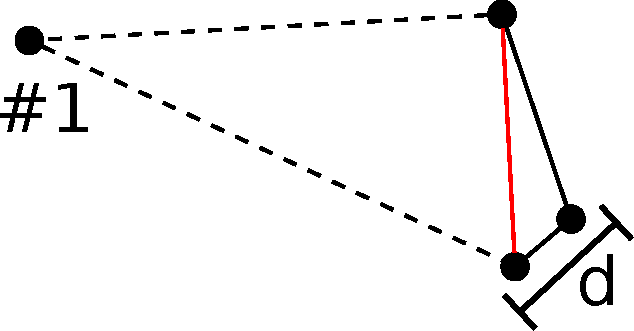
\includegraphics[width=0.5\textwidth]{drawing.pdf}
    \caption{Illustration of the smallest 1-tree and optimal TCP of the graph containing $v_1, v_2, v_3$ and $v_4$}
    \label{fig:ex12}
\end{figure}

